\documentclass[conference,a4paper]{IEEEtran}
\usepackage[utf8]{inputenc}
\usepackage[T1]{fontenc}
\usepackage[provide=*,spanish]{babel}
\usepackage{amsmath,amssymb,graphicx,booktabs,tabularx,array,microtype,cite,flushend}
\usepackage{tikz}
\usetikzlibrary{arrows.meta,positioning}
\usepackage[hidelinks]{hyperref}
\addto\captionsspanish{\renewcommand{\abstractname}{Resumen}\renewcommand{\refname}{Referencias}\renewcommand{\tablename}{TABLA}\renewcommand{\figurename}{Fig.}}
\renewcommand{\IEEEkeywordsname}{Palabras clave}
\hypersetup{pdftitle={Optimización de capacidad y balanceo de carga en un centro de datos cloud mediante simulación},pdfauthor={Franco Salvador Paredes Zamora; Jesús Alberto Briceño Vera; Gonzalo Gilmar Flores Cruz}}
\setlength{\emergencystretch}{1.2em}
\newcolumntype{Y}{>{\raggedright\arraybackslash}X}
\newcommand{\inputrows}[1]{\csname @@input\endcsname #1 }
\newcommand{\valW}{0.2006}
\newcommand{\errW}{0.29}
\newcommand{\valL}{1.0035}
\newcommand{\errL}{0.35}
\newcommand{\valrho}{0.5008}
\newcommand{\errrho}{0.15}
\newcommand{\ElegidaVM}{8}
\newcommand{\ElegidaPolitica}{MP}
\newcommand{\ElegidaCosto}{0.9589}
\newcommand{\ElegidaA}{99.940}
\newcommand{\ElegidaG}{99.727}
\newcommand{\ElegidaP}{0.494}
\newcommand{\ElegidaLCBA}{99.930}
\newcommand{\ElegidaLCBG}{99.577}
\newcommand{\AltaDif}{-0.468}
\newcommand{\AltaLo}{-0.479}
\newcommand{\AltaHi}{-0.457}
\newcommand{\AltaRed}{45.990}
\newcommand{\PicoDif}{-0.151}
\newcommand{\PicoLo}{-0.172}
\newcommand{\PicoHi}{-0.130}
\newcommand{\PicoRed}{23.411}

\begin{document}
\title{Optimización de capacidad y balanceo de carga en un centro de datos cloud mediante simulación}
\author{
\IEEEauthorblockN{Franco Salvador Paredes Zamora}
\IEEEauthorblockA{Ingeniería de Sistemas\\Universidad Católica de Santa María\\Arequipa, Perú}
\and
\IEEEauthorblockN{Jesús Alberto Briceño Vera}
\IEEEauthorblockA{Ingeniería de Sistemas\\Universidad Católica de Santa María\\Arequipa, Perú}
\and
\IEEEauthorblockN{Gonzalo Gilmar Flores Cruz}
\IEEEauthorblockA{Ingeniería de Sistemas\\Universidad Católica de Santa María\\Arequipa, Perú}}
\maketitle
\begin{abstract}
Se evaluó el compromiso entre costo y calidad de servicio en seis configuraciones cloud: cuatro, seis u ocho máquinas virtuales con Round Robin o menor cantidad de solicitudes pendientes. La simulación representa CPU, memoria reservada, colas finitas, plazos y fallos de host. Se ejecutaron 1.080 experimentos con tres cargas, dos condiciones de fallo y 30 réplicas por combinación; la implementación se contrastó con M/M/1 y pruebas deterministas. Entre las alternativas factibles, \ElegidaVM{} máquinas virtuales con \ElegidaPolitica{} minimizaron el costo y ganaron el desempate por latencia. Su costo fue \ElegidaCosto{} unidades monetarias por ejecución y su menor cumplimiento de dos segundos fue \ElegidaG{}\,\%. La selección se limita al modelo sintético y no certifica un servicio real.
\end{abstract}
\begin{IEEEkeywords}
optimización de operaciones, simulación de eventos discretos, teoría de colas, cloud computing, disponibilidad, balanceo de carga.
\end{IEEEkeywords}
\section{Introducción}
Un servicio digital recibe solicitudes cuya demanda varía en el tiempo. Si la capacidad de procesamiento resulta insuficiente, aumentan las colas, los tiempos de respuesta y los rechazos. Contratar más recursos puede reducir esa degradación, pero incrementa el costo incluso durante períodos de baja demanda. La decisión de capacidad es, por tanto, un problema de optimización de operaciones con restricciones de servicio.

El cloud computing proporciona acceso bajo demanda a recursos compartidos, elasticidad y medición del uso, según NIST \cite{nist}. Estas características no suprimen los límites de CPU, memoria o concurrencia. La virtualización agrega una capa de asignación entre los servidores físicos y las aplicaciones; varias máquinas virtuales (VMs) alojadas en un mismo host comparten el riesgo de perderse cuando ese equipo falla.

La pregunta de investigación es: ¿qué combinación de cantidad de VMs y política de balanceo minimiza el costo de aprovisionamiento, manteniendo objetivos de éxito y tiempo de respuesta ante cambios de demanda y el fallo de un host? El objetivo general consiste en seleccionar esa combinación mediante una evaluación exhaustiva de alternativas con simulación de eventos discretos.

El trabajo aporta un modelo explícito de capacidad y colas, una formulación de costo con restricciones de servicio y un experimento reproducible que vincula la decisión con resultados medidos. Se trata de una evaluación académica de políticas conocidas; no se propone un algoritmo nuevo ni se afirma optimalidad fuera del conjunto de configuraciones estudiado.

\section{Fundamentos y trabajos relacionados}
\subsection{Simulación y optimización de recursos}
CloudSim estableció un marco para modelar infraestructuras cloud y evaluar algoritmos de aprovisionamiento sin contratar un despliegue equivalente \cite{cloudsim}. En este trabajo se empleó SimPy, cuyo calendario de eventos y representación de procesos permiten expresar los cambios de estado de una simulación discreta \cite{simpy}. Los hosts, las VMs, la facturación y las reglas de fallo fueron implementados como componentes del modelo, no como funcionalidades de una nube real ejecutada por SimPy.

La optimización mediante simulación utiliza las salidas del modelo para comparar decisiones cuyo desempeño no se conoce analíticamente. Cuando las alternativas son pocas, es posible evaluarlas todas; Nelson presenta el contexto de selección entre sistemas simulados \cite{nelson}. Aquí se realizó enumeración finita con restricciones estimadas, sin aplicar un procedimiento con garantía formal de probabilidad de selección correcta.

\subsection{Colas y calidad de servicio}
El tiempo de respuesta se descompone en:
\begin{equation}
R=W_q+S+d,
\label{eq:respuesta}
\end{equation}
donde $W_q$ es la espera, $S$ el servicio de CPU y $d$ el retardo de red. La utilización nominal para $k$ puestos homogéneos y tasa de servicio $\mu$ por puesto es $\rho=\lambda/(k\mu)$. En M/M/1 con cola ilimitada y $\rho<1$, se obtiene $W=1/(\mu-\lambda)$ y $L=\lambda W$ \cite{colas}. La espera crece de manera no lineal al acercarse la demanda a la capacidad.

Las fórmulas estacionarias no describen directamente un sistema con demanda variable, colas separadas, plazos y fallos. Además, Round Robin transforma el proceso de llegada a cada VM, por lo que no se supone que cada cola individual tenga llegadas Poisson. La teoría sirve como referencia y como caso de verificación independiente.

\subsection{Balanceo y disponibilidad}
Round Robin (RR) distribuye por turnos entre destinos elegibles. La política de menor cantidad de solicitudes pendientes (MP) considera solicitudes en ejecución y espera. AWS documenta algoritmos de reparto por turnos y por solicitudes pendientes \cite{aws}; la implementación estudiada se define mediante sus propias reglas y no pretende reproducir completamente un balanceador comercial.

La disponibilidad por solicitudes se mide como la fracción de peticiones correctas, mientras que la latencia representa otra dimensión del servicio \cite{sre}. Mantener ambos indicadores evita considerar suficiente una respuesta que termina correctamente después del plazo deseado. La disponibilidad de un host, la del servicio completo y la conservación de datos son conceptos distintos.

\section{Modelo y formulación de optimización}
\subsection{Arquitectura y recursos}
Se modeló un servicio limitado principalmente por CPU sobre cuatro hosts físicos. Cada host dispone de ocho núcleos y 16 GiB de RAM. Cada VM reserva dos vCPU y 4 GiB; cada vCPU atiende una solicitud a la vez, sin compartir el puesto durante su ejecución. La reserva de memoria se satisface por construcción para los tamaños evaluados; no se verifica dinámicamente ni se modela como consumo variable por solicitud.

La ubicación es cíclica: la VM $i$, numerada desde uno, se asigna al host $1+((i-1)\bmod4)$. Para $c=4,6,8$, las distribuciones son $(1,1,1,1)$, $(2,2,1,1)$ y $(2,2,2,2)$ VMs. Por tanto, la caída del host 1 elimina una, dos y dos VMs respectivamente. Esta diferencia forma parte del escenario definido, no de un efecto atribuible exclusivamente al balanceo.

\begin{figure}[t]
\centering
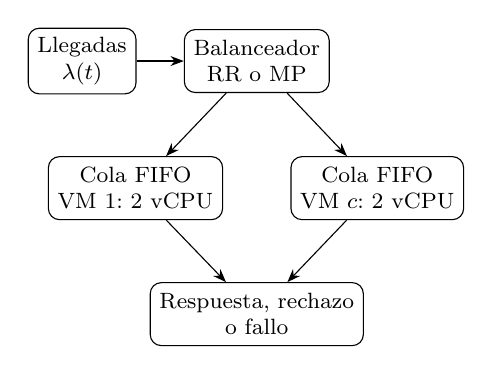
\begin{tikzpicture}[>=Stealth,box/.style={draw,rounded corners,align=center,font=\footnotesize,minimum height=8mm},node distance=6mm]
\node[box] (a) {Llegadas\\$\lambda(t)$};
\node[box,right=of a] (b) {Balanceador\\RR o MP};
\node[box,below left=8mm and -5mm of b] (q1) {Cola FIFO\\VM 1: 2 vCPU};
\node[box,below right=8mm and -5mm of b] (q2) {Cola FIFO\\VM $c$: 2 vCPU};
\node[box,below=24mm of b] (r) {Respuesta, rechazo\\o fallo};
\draw[->] (a)--(b);\draw[->] (b)--(q1);\draw[->] (b)--(q2);
\draw[->] (q1)--(r);\draw[->] (q2)--(r);
\end{tikzpicture}
\caption{Flujo lógico del modelo. Las VMs se ubican en cuatro hosts físicos; cada VM mantiene una cola independiente.}
\label{fig:modelo}
\end{figure}

Sea $z_{ih}$ la asignación binaria de una VM a un host. La ubicación satisface:
\begin{align}
\sum_h z_{ih}&=1 &&\forall i,\\
\sum_i v_i z_{ih}&\leq V_h &&\forall h,\\
\sum_i m_i z_{ih}&\leq M_h &&\forall h,
\end{align}
donde $v_i,m_i$ son los recursos de la VM y $V_h,M_h$ los del host. La ubicación permanece fija durante la ejecución y no se optimiza en este estudio.

\subsection{Solicitudes y reglas de atención}
Las llegadas siguen un proceso Poisson por tramos. Los servicios son independientes y exponenciales con media de 0,10 s; el retardo de red total es fijo, de 0,02 s, y se aplica después del servicio sin ocupar CPU. Cada VM dispone de una cola FIFO con hasta 100 solicitudes esperando, además de dos en ejecución.

RR utiliza un cursor circular sobre las VMs elegibles. MP selecciona el menor valor de $n_i^{\mathrm{ejec}}+n_i^{\mathrm{cola}}$, resolviendo empates mediante un cursor circular. No utiliza la duración futura de los trabajos. Si la VM seleccionada tiene la cola llena, la solicitud se rechaza sin segundo intento. Una solicitud vence definitivamente a los 10 s desde su llegada; su espera o ejecución se cancela y libera recursos. Las respuestas correctas de hasta dos segundos cumplen el objetivo de rapidez.

Ante un fallo, se pierden las solicitudes activas en las VMs afectadas, incluidas las respuestas aún pendientes del retardo de red. La detección tarda cinco segundos; durante ese intervalo las VMs continúan elegibles y los nuevos envíos fallan. MP conserva, para ellas, el último número conocido de solicitudes pendientes, sin acceder al estado real del host. Tras la detección se excluyen y se reincorporan al recuperarse el host. No se modelaron reintentos, migración ni autoescalado.

La Fig.~\ref{fig:pseudocodigo} resume el procesamiento por eventos. El fallo y el vencimiento interrumpen el trabajo en el instante en que ocurren; no se comprueban únicamente después de completar el servicio. Una solicitud finalizada no cambia de resultado si después se procesa un evento que había quedado programado para ella.

\begin{figure}[t]
\centering\footnotesize
\begin{tabularx}{\columnwidth}{@{}>{\raggedright\arraybackslash}p{.18\columnwidth}Y@{}}
\toprule
\textbf{Evento} & \textbf{Pseudocódigo de la acción}\\\midrule
Llegada de $r$ & Seleccionar VM según RR o MP. Si no existe destino elegible o está caído: registrar fallo y terminar. Si no hay CPU libre y la cola tiene 100 solicitudes: rechazar y terminar. En otro caso, registrar $r$ activa y programar su vencimiento en $t_r+10$ s. Iniciar CPU si hay un puesto libre; de lo contrario, encolar en FIFO.\\[3pt]
Fin de CPU & Si $r$ sigue ejecutándose: liberar su puesto, pasar $r$ a respuesta pendiente y programar su entrega tras 0,02 s; iniciar la primera solicitud válida de la cola, si existe.\\[3pt]
Entrega & Si $r$ sigue pendiente de respuesta: registrar correcta, medir $R$ y contar cumplimiento si $R\leq2$ s; retirar $r$ de las activas.\\[3pt]
Vencimiento & Si $r$ sigue activa: cancelar su espera, ejecución o respuesta pendiente y registrar vencida. Si ocupaba CPU, liberar el puesto e iniciar la siguiente solicitud válida.\\[3pt]
Fallo de host & Conservar la ocupación conocida para MP y marcar sus VMs caídas. Finalizar inmediatamente sus solicitudes activas como fallidas; vaciar las colas afectadas.\\[3pt]
Detección y recuperación & Al detectar el fallo, excluir las VMs del reparto. Al recuperarse el host, marcarlas operativas y elegibles.\\\bottomrule
\end{tabularx}
\caption{Pseudocódigo del simulador por eventos. Las verificaciones de estado evitan contar dos veces una solicitud y permiten cancelar CPU o espera sin aguardar al fin del servicio.}
\label{fig:pseudocodigo}
\end{figure}

\subsection{Decisiones, costo y restricciones}
La decisión es $x=(c,b)$, con $c\in\{4,6,8\}$ VMs y $b\in\{\mathrm{RR},\mathrm{MP}\}$. Sea $\mathcal S$ el conjunto de seis escenarios de carga y fallo. El problema es:
\begin{align}
\min_{x\in\mathcal X}\quad&C(x)=(p_{\mathrm{VM}}c+p_{\mathrm{LB}})T,\label{eq:objetivo}\\
\text{sujeto a}\quad&A_s(x)\geq0,99 &&\forall s\in\mathcal S,\label{eq:disp}\\
&G_s(x)\geq0,95 &&\forall s\in\mathcal S,\label{eq:rapidez}
\end{align}
con $\mathcal X=\{4,6,8\}\times\{\mathrm{RR},\mathrm{MP}\}$. $A_s$ es la probabilidad de respuesta correcta antes de 10 s y $G_s$ la de respuesta correcta en hasta 2 s; se estimaron como promedios de proporciones por réplica. En cada réplica:
\begin{equation}
\widehat A=\frac{N_{\mathrm{correctas}}}{N_{\mathrm{ofrecidas}}},\qquad
\widehat G=\frac{N_{\mathrm{correctas},R\leq2\,\mathrm{s}}}{N_{\mathrm{ofrecidas}}}.
\end{equation}
Rechazos, vencimientos y fallos permanecen en el denominador. Se emplearon tarifas sintéticas de 0,10 unidades monetarias (u. m.) por VM-hora y 0,02 u. m. por hora de balanceador. El costo representa aprovisionamiento desde la perspectiva del consumidor, incluso durante un fallo; no representa energía, inversión ni operación física del centro de datos. Almacenamiento y transferencia variables quedaron fuera del alcance.

Las restricciones se evaluaron sobre medias muestrales en cada escenario. Los intervalos de confianza permiten evaluar incertidumbre, sin convertir esa regla en una garantía simultánea. Entre alternativas factibles se eligió el menor costo; en empate, el menor p95 medio en el escenario más desfavorable. La búsqueda exhaustiva garantiza revisar las seis alternativas, no conocer sin error sus desempeños verdaderos.

\section{Metodología experimental}
\subsection{Diseño factorial y control de entradas}
Se evaluaron tres tamaños, dos políticas, tres perfiles de demanda y dos condiciones de fallo. Cada combinación tuvo 30 réplicas: $3\times2\times3\times2\times30=1.080$ ejecuciones.

\begin{table}[t]
\caption{Parámetros del experimento principal}
\label{tab:parametros}
\centering\footnotesize
\begin{tabularx}{\columnwidth}{@{}p{.36\columnwidth}Y@{}}\toprule
Parámetro & Valor\\\midrule
Infraestructura & 4 hosts, 8 núcleos y 16 GiB por host\\
VMs & 4, 6 u 8; 2 vCPU y 4 GiB por VM\\
Cola por VM & FIFO; 100 solicitudes esperando\\
Servicio por puesto & Exponencial; media 0,10 s\\
Retardo de red & 0,02 s fijo, sin ocupar CPU\\
Objetivo / vencimiento & 2 s / 10 s desde la llegada\\
Calentamiento & 600 s con la tasa inicial\\
Medición / seguimiento & 3.600 s / 10 s\\
Fallo / detección & Host 1: 120 s / 5 s\\
Réplicas & 30 por combinación\\\bottomrule
\end{tabularx}
\end{table}

La carga baja mantuvo 40 solicitudes/s y la alta, 72. El perfil con pico utilizó 40, 120 y 40 solicitudes/s en tres tramos de 1.200 s. Cada perfil se ejecutó sin fallo y con caída del host 1 entre los segundos 1.800 y 1.920 de medición. Las capacidades nominales sin fallo fueron 80, 120 y 160 solicitudes/s; con fallo, 60, 80 y 120. Una intensidad nominal igual a uno no asegura buen servicio durante el intervalo afectado.

Se utilizaron dos flujos aleatorios separados para llegadas y servicio, derivados de \texttt{SeedSequence} de NumPy con base 20261029, índice de réplica e índice de carga. Cada solicitud recibió su trabajo antes de aplicar el balanceo. Para una misma carga y réplica se reutilizó la traza completa en todas las alternativas y condiciones de fallo; su identidad se registró mediante SHA-256. Este acoplamiento evita atribuir a la política diferencias causadas por entradas distintas.

La medición por solicitudes incluye las llegadas durante la ventana observada, con seguimiento hasta su terminación o vencimiento. Las solicitudes del calentamiento no forman parte de esa cohorte, aunque sí pueden ocupar recursos al iniciar la ventana. Para el costo se usó un horizonte común de $T=(600+3.600+10)/3.600=1,16944$ horas, sin asumir que una hora simulada equivale a una hora de ejecución del programa.

\subsection{Indicadores e incertidumbre}
Se registraron $A$, $G$, latencia media y p95 de respuestas correctas, espera media de esas respuestas, longitud de cola ponderada por tiempo y utilización. La cola media del sistema es:
\begin{equation}
\overline Q=\frac{1}{H}\int_0^H\sum_{i=1}^{c}Q_i(t)\,dt,
\end{equation}
donde $H=3.600$ s. La utilización es el tiempo de vCPU ocupado dividido entre $2cH$; incluye la capacidad contratada durante los fallos en el denominador. Las integrales se actualizan exactamente en cada cambio de estado, no mediante el muestreo de las figuras.

El throughput contabiliza respuestas correctas finalizadas dentro de la ventana dividido entre $H$; difiere de la proporción de éxito de la cohorte, que contempla el seguimiento. El p95 se calcula por réplica sobre respuestas correctas; los errores se reflejan en $A$ y $G$. Por ello no se utiliza una baja latencia condicionada a éxitos como evidencia suficiente de buen servicio.

Para cada indicador se calculó un intervalo puntual del 95\,\%:
\begin{equation}
\bar y\pm t_{0,975;29}\frac{s_y}{\sqrt{30}}.
\end{equation}
El p95 informado es el promedio de los p95 de las réplicas. Las diferencias MP--RR se analizaron por semilla mediante intervalos pareados. No se trataron las solicitudes de una misma ejecución como observaciones independientes para estimar la incertidumbre entre réplicas. Los intervalos son aproximados y no están ajustados para comparaciones múltiples.

\subsection{Verificación y contraste analítico}
Se distinguió la verificación del programa del alcance de su validación, siguiendo la separación conceptual discutida por Sargent \cite{sargent}. Se implementaron diez pruebas deterministas para comprobar FIFO, capacidad de cola, liberación de CPU por vencimiento, eliminación de esperas vencidas, fallo y detección, retardo sin retener CPU, cohorte y seguimiento, integrales de estado, selección MP y reproducibilidad de trazas.

Cada ejecución comprobó además la identidad entre solicitudes ofrecidas y sus cuatro estados terminales excluyentes: correctas, rechazadas, vencidas y fallidas. Se verificó que ninguna VM excediera dos solicitudes simultáneas y que no quedaran solicitudes activas al terminar el seguimiento.

El contraste analítico utilizó M/M/1 con $\lambda=5$, $\mu=10$, un puesto, cola ilimitada, sin red, plazos ni fallos. Se realizaron 30 réplicas adicionales con 1.000 s de calentamiento y 10.000 s de medición. Las referencias son $W=0,20$ s, $L=1$ y $\rho=0,5$. Esta prueba acredita coherencia con un caso conocido; no valida el modelo completo contra un centro de datos real.

\section{Resultados}
\subsection{Contraste del simulador}
Las diez pruebas deterministas finalizaron correctamente. El contraste M/M/1 produjo los valores de la Tabla~\ref{tab:validacion}; los tres intervalos contienen sus referencias teóricas. Los errores relativos fueron inferiores al 0,4\,\%, lo que respalda el funcionamiento de la atención y las mediciones en el caso simplificado.

\begin{table}[t]
\centering\footnotesize
\caption{Contraste analítico M/M/1: 30 réplicas}
\label{tab:validacion}
\begin{tabular}{@{}lrrrr@{}}\toprule
Métrica & Teoría & Simulación & IC 95\,\% & Error (\%)\\\midrule
\inputrows{resultados/tabla_validacion.tex}
\bottomrule\end{tabular}
\end{table}

\subsection{Demanda, colas y distribución de trabajo}
La Tabla~\ref{tab:rendimiento} muestra los escenarios sin fallo. Las diferencias entre tamaños deben interpretarse junto con la carga: una configuración puede ser suficiente durante demanda baja y resultar inadecuada durante el pico. El aumento de capacidad no altera los tiempos de servicio generados; modifica la contención y la espera.

Con cuatro VMs y carga alta, MP redujo el p95 medio en \AltaRed{}\,\% respecto a RR. La diferencia pareada MP--RR fue \AltaDif{} s, con IC 95\,\% [\AltaLo{}, \AltaHi{}]. Durante el pico, cuatro VMs no aportaron capacidad suficiente y ambas políticas incumplieron el objetivo, pese a que la utilización media de toda la ventana no alcanzó el 100\,\%.

\begin{table}[t]
\centering\footnotesize
\caption{Rendimiento sin fallo: medias de 30 réplicas}
\label{tab:rendimiento}
\begin{tabular}{@{}lrlrrrr@{}}\toprule
Carga & VMs & Pol. & p95 (s) & $\overline Q$ & CPU (\%) & $G$ (\%)\\\midrule
\inputrows{resultados/tabla_rendimiento.tex}
\bottomrule\end{tabular}
\end{table}

La Fig.~\ref{fig:latencia} compara el p95 del perfil con pico, con y sin fallo. MP utiliza la ocupación observada para evitar destinos con mayor acumulación de trabajo; RR conserva la secuencia de turnos. Ambas políticas están limitadas por la capacidad total, de modo que una distribución diferente no elimina un déficit sostenido de procesamiento.

\begin{figure}[t]
\centering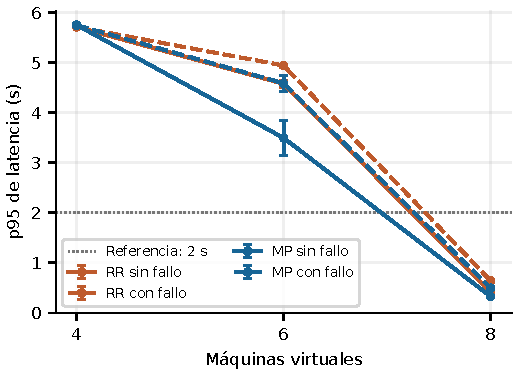
\includegraphics[width=\columnwidth]{figuras/latencia.pdf}
\caption{Latencia en el perfil con pico. Barras: IC puntual del 95\,\% para la media de p95 entre réplicas. La línea de 2 s es una referencia visual; la restricción formal se evalúa con $G$.}
\label{fig:latencia}
\end{figure}

\subsection{Fallo del host y evolución temporal}
La Fig.~\ref{fig:evolucion} presenta una réplica con entradas comunes y distintas configuraciones. El intervalo sombreado identifica el fallo del host 1. La pérdida de capacidad se superpone a la fase de demanda máxima; las colas muestran la capacidad del sistema para absorber y eliminar la acumulación. La ocupación de CPU se interpreta con relación a la capacidad disponible y a la contratada.

\begin{figure*}[t]
\centering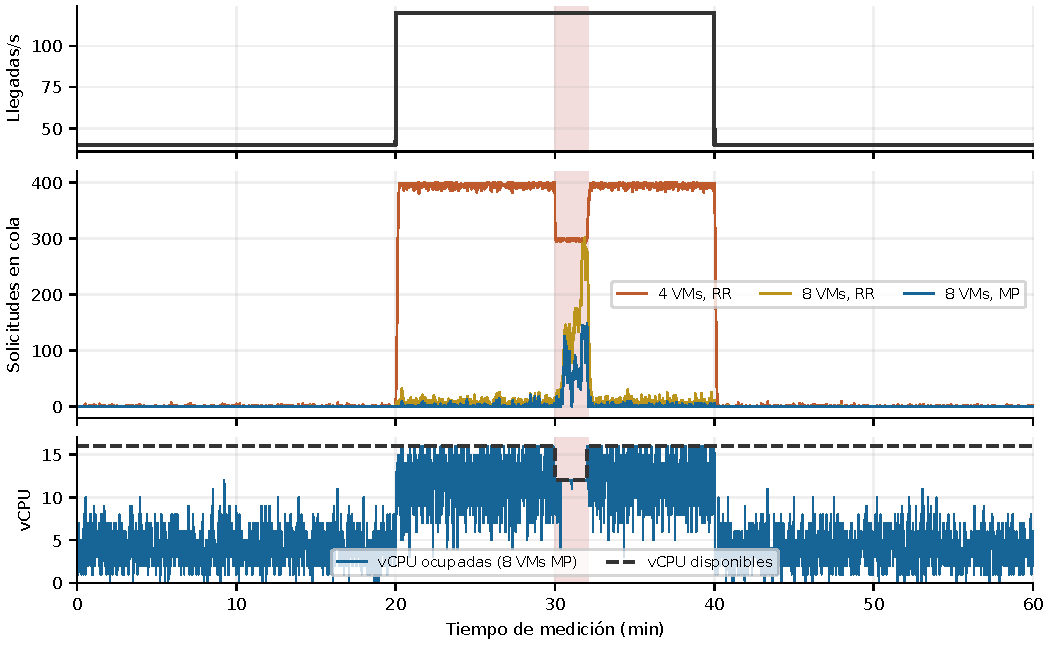
\includegraphics[width=.91\textwidth]{figuras/evolucion.pdf}
\caption{Evolución de una réplica del perfil con pico y fallo, semilla 0. La demanda aumenta en el minuto 20 y disminuye en el 40; el host 1 está caído entre los minutos 30 y 32. Las series se muestrean cada segundo para exposición y no sustituyen el análisis de las 30 réplicas.}
\label{fig:evolucion}
\end{figure*}

\subsection{Selección de la alternativa de menor costo}
La Tabla~\ref{tab:seleccion} resume, para cada alternativa, el mínimo éxito, el mínimo cumplimiento de rapidez y el máximo p95 medio entre los seis escenarios. Los extremos de una fila pueden corresponder a escenarios diferentes. Una alternativa es factible únicamente cuando todas sus medias de escenario satisfacen las restricciones.

\begin{table*}[t]
\centering\small
\caption{Evaluación exhaustiva de alternativas; costo sintético por horizonte común}
\label{tab:seleccion}
\begin{tabular}{@{}rcrrrrc@{}}\toprule
VMs & Política & Costo (u. m.) & Mín. $A$ (\%) & Mín. $G$ (\%) & Máx. p95 (s) & Factible\\\midrule
\inputrows{resultados/tabla_seleccion.tex}
\bottomrule\end{tabular}
\end{table*}

La regla de decisión seleccionó \ElegidaVM{} VMs y \ElegidaPolitica{}, con costo de \ElegidaCosto{} u. m. por ejecución. Su menor éxito fue \ElegidaA{}\,\%, su menor cumplimiento de dos segundos fue \ElegidaG{}\,\% y su máximo p95 medio fue \ElegidaP{} s. El costo depende del número de VMs, no de la política, por lo que el desempate mediante latencia distingue alternativas con igual aprovisionamiento.

Ambas políticas con ocho VMs resultaron factibles. En el pico con fallo, MP redujo el p95 medio en \PicoRed{}\,\% frente a RR; la diferencia pareada fue \PicoDif{} s, con IC 95\,\% [\PicoLo{}, \PicoHi{}]. Para la alternativa seleccionada, los mínimos límites inferiores puntuales fueron \ElegidaLCBA{}\,\% en éxito y \ElegidaLCBG{}\,\% en rapidez, por encima de sus respectivos umbrales.

\begin{figure}[t]
\centering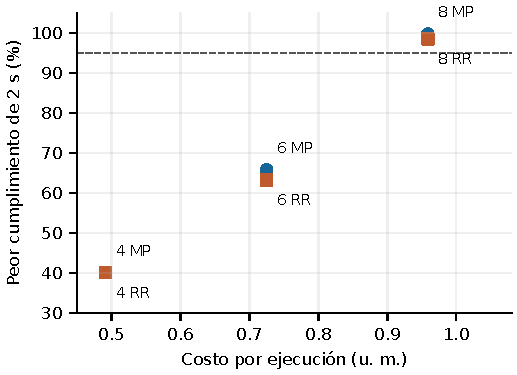
\includegraphics[width=\columnwidth]{figuras/costo_servicio.pdf}
\caption{Compromiso costo--rapidez. Cada punto es una configuración; el eje vertical recoge el peor $G$ medio entre escenarios. La línea discontinua marca el objetivo del 95\,\%; también se exige $A\geq99\,\%$.}
\label{fig:costo}
\end{figure}

Los CSV conservan las métricas por réplica. Los resúmenes, las diferencias pareadas y la selección se generan por programa; LaTeX importa directamente las tablas calculadas.

\subsection{Costo incremental de la capacidad}
Con el horizonte común de $T=1,16944$ h, cada VM adicional agrega \CostoVMAdicional{} u. m. por ejecución y el balanceador aporta \CostoBalanceador{} u. m. fijas. Los porcentajes siguientes se calcularon con los costos originales, antes de redondearlos para su presentación.

Pasar de seis a ocho VMs incrementó el costo de \CostoSeis{} a \CostoOcho{} u. m., un \AumentoSeisOcho{}\,\%. En la política MP, el peor cumplimiento de dos segundos aumentó de \GSeisMP{}\,\% a \ElegidaG{}\,\%. Dentro de los tamaños evaluados, ocho VMs fue la menor capacidad que satisfizo simultáneamente las restricciones~\eqref{eq:disp} y~\eqref{eq:rapidez} en todos los escenarios.

Reducir de ocho a cuatro VMs ahorra \AhorroOchoCuatro{}\,\%, pero con MP el peor cumplimiento cae a \GCuatroMP{}\,\% e incumple las restricciones. La selección considera costo de aprovisionamiento y factibilidad; no estima rentabilidad total, pues no incluye penalizaciones monetarias por errores o demora.

\section{Discusión}
\subsection{Interpretación desde optimización de operaciones}
El experimento separa capacidad y distribución: comparar RR con MP para un mismo número de VMs estudia el balanceo; comparar tamaños bajo una misma política estudia el aprovisionamiento. La decisión final combina ambos factores con restricciones explícitas. El criterio no consiste en maximizar utilización: una utilización elevada puede acompañarse de colas y deterioro del servicio.

El mínimo costo aislado favorece contratar menos VMs. Las restricciones evitan aceptar ese ahorro cuando se consigue a costa de errores o espera excesiva. Por otro lado, dos configuraciones con el mismo precio pueden tener distribuciones distintas de latencia. Esta separación explica por qué una política de balanceo puede mejorar la calidad sin modificar la factura del modelo.

Los fallos exhiben el efecto de la ubicación física. Duplicar VMs dentro del mismo host no elimina el dominio de fallo compartido. Con seis VMs, la caída del host 1 elimina dos de ellas, mientras que con cuatro elimina una. Por ello los resultados no demuestran que cualquier crecimiento de capacidad produzca una mejora proporcional bajo todos los fallos posibles.

\subsection{Limitaciones y alcance de la evidencia}
La carga es sintética y exponencial; no representa trazas de una organización ni distribuciones con colas pesadas. Las vCPU son puestos homogéneos, sin virtualización detallada, interferencia de vecinos o degradación por concurrencia. La RAM es una restricción de reserva; disco y red no generan contención. Las tarifas son ilustrativas y no permiten estimar una factura comercial.

Se evaluó un fallo controlado de un host, con una regla concreta de detección. No se estimaron tasas de fallo, tiempos medios entre fallos ni disponibilidad anual. El balanceador no falla y no existen reintentos. El autoescalado y sus demoras no forman parte de las políticas estudiadas.

Generalizar a producción requiere calibración con mediciones, sensibilidad a distribuciones y tarifas, y una política de inferencia compatible con el riesgo de decisión. Los intervalos puntuales no garantizan simultáneamente el cumplimiento en todos los escenarios.

\section{Reproducibilidad y demostración}
El repositorio contiene código, pruebas, CSV por réplica, metadatos, huellas de trazas y figuras. Se utilizó Python con SimPy 4.1.1 y dependencias fijadas en \texttt{requirements.txt}; el README documenta los comandos de reproducción.

La demostración reproduce las series mediante \texttt{python -m simulacion.demostrar}, con pausa y selección temporal. Permite observar demanda, colas y capacidad durante el fallo. La evidencia estadística corresponde a las réplicas, no a una única animación.

\section{Conclusiones}
Se implementó un modelo de eventos discretos que relaciona servidores físicos, VMs, colas, balanceo, fallos y costo de aprovisionamiento. Su coherencia se verificó mediante diez pruebas deterministas y un contraste M/M/1 cuyos errores relativos fueron menores al 0,4\,\%.

La evaluación de seis alternativas bajo seis escenarios, con 30 réplicas por combinación, permitió seleccionar \ElegidaVM{} VMs con \ElegidaPolitica{} mediante costo y desempate por p95. La alternativa seleccionada alcanzó un cumplimiento mínimo de \ElegidaG{}\,\% para respuestas correctas en hasta dos segundos y un costo de \ElegidaCosto{} u. m. por horizonte experimental.

La simulación convirtió una decisión de recursos en una comparación cuantificable con restricciones de servicio. La conclusión se limita al modelo y al conjunto evaluado: no acredita una política universal, un SLA comercial ni la disponibilidad de una infraestructura real.

\bibliographystyle{IEEEtran}
\bibliography{referencias}
\end{document}
